%%%%%%%%%%%%%%%%%%%%%%%%%%%%%%%%%%%%%%%%%%%%%%%
%%%This is a science homework template. Modify the preamble to suit your needs.
%%%%%%%%%%%%%%%%%%%%%%%%%%%%%%%%%%%%%%%%%%%%%%%%

\documentclass[12pt]{article}

\usepackage{amssymb,amsmath,amsthm}
\usepackage[margin=1.25in]{geometry}
\usepackage{graphicx,ctable,booktabs, tikz}
\usepackage{listings} %for inserting code snippets
%%%%%%%%%%%%%%%%%Quantum Circuist%%%%%%%%%%%%%%%%%%%%%%
\usepackage{etex}
\usepackage[all]{xy}
\SelectTips{em}{}
\input{Qcircuit}
\vfuzz2pt % Don't report over-full v-boxes if over-edge is small
%\usepackage[all]{xy}
%%%%%%%%%%%%%%%%%%%%%%%%%%%%%%%%%%%%%%%%%%%%%%%%%%%%%%%
\usepackage{multicol}

\newcommand{\<}{\langle}
\renewcommand{\>}{\rangle}
\newcommand{\C}{\mathbb{C}}
\newcommand{\cA}{\mathcal{A}}
\newcommand{\cB}{\mathcal{B}}
\newcommand{\cC}{\mathcal{C}}
\newcommand{\cE}{\mathcal{E}}
\newcommand{\cF}{\mathcal{F}}
\newcommand{\cH}{\mathcal{H}}
\newcommand{\cK}{\mathcal{K}}
\newcommand{\cM}{\mathcal{M}}
\newcommand{\cR}{\mathcal{R}}
\newcommand{\cU}{\mathcal{U}}
\newcommand{\cV}{\mathcal{V}}
\newcommand{\cZ}{\mathcal{Z}}
\newcommand{\E}{\mathrm{\mathbf{E}}}
\newcommand{\Var}{\mathrm{\mathbf{Var}}}
\newcommand{\EE}[1]{\E\left(#1\right)}
\newcommand{\VV}[1]{\Var\left(#1\right)}
\newcommand{\s}{\mathrm{span}}
\newcommand{\R}{\mathbb{R}}
\renewcommand{\sim}{\mathrm{sim}}
\renewcommand{\prec}{\mathrm{prec}}
\newcommand{\fail}{\mathrm{fail}}
\newcommand{\median}{\mathrm{median}}
\newcommand{\anc}{\mathrm{anc}}

\renewcommand{\labelitemii}{$\circ$}

% \newcommand{\ket}[1]{\left| #1\right\rangle}      % ket vector
% \newcommand{\bra}[1]{\left\langle #1\right|}      % bra vector
\newcommand{\kets}[1]{| #1 \rangle}                 % small ket vector
\newcommand{\bras}[1]{\langle #1 |}                 % small bra vector
\newcommand{\braket}[2]{\langle #1 | #2 \rangle}         % <x|y>
\newcommand{\ii}{\mathbb{I}}

% the I with two vertical lines
\newcommand{\twonorm}[1]{\left\| #1\right\|_2}        % norm
\newcommand{\inftynorm}[1]{\left\| #1\right\|_\infty}
\newcommand{\norms}[1]{\big\| #1\big\|}          % norm

\newcommand{\tr}{\mathrm{tr}}
%\newcommand{\qed}{\hfill $\square$}
\newtheorem{definition}{Definition}
\newtheorem{theorem}{Theorem}
\newtheorem{lemma}{Lemma}
\newtheorem{proposition}{Proposition}
\newtheorem{cor}{Corollary}
\newtheorem{remark}{Remark}


\makeatletter
\newenvironment{problem}{\@startsection
       {section}
       {1}
       {-.2em}
       {-3.5ex plus -1ex minus -.2ex}
       {2.3ex plus .2ex}
       {\pagebreak[3]
       \large\bf\noindent{Problem }
       }
       }
       {%\vspace{1ex}\begin{center} \rule{0.3\linewidth}{.3pt}\end{center}}
       \begin{center}\large\bf \end{center}}
\makeatother


%
%Fancy-header package to modify header/page numbering
%
\usepackage{fancyhdr}
\pagestyle{fancy}
%\addtolength{\headwidth}{\marginparsep} %these change header-rule width
%\addtolength{\headwidth}{\marginparwidth}
\lhead{Problem \thesection}
\chead{}
\rhead{\thepage}
\lfoot{\small\scshape CS 518}
\cfoot{}
\rfoot{\footnotesize }
\renewcommand{\headrulewidth}{.3pt}
\renewcommand{\footrulewidth}{.3pt}
\setlength\voffset{-0.25in}
\setlength\textheight{648pt}

%%%%%%%%%%%%%%%%%%%%%%%%%%%%%%%%%%%%%%%%%%%%%%%

\def\ket#1{\big|{#1}\big>}
\def\bra#1{\big<{#1}\big|}
\def\braket#1#2{\big<{#1}\big|{#2}\big>}
\def\ketbra#1{\big|{#1}\big>\big<{#1}\big|}
\def\sqtwo{\sqrt{2}}
\pagestyle{empty}
\begin{document}
\centerline{\bf CSC518  \hfill HW \#2}
\centerline{\bf NAME: Alexander Jansing and Brittany Zeo \hfill Wed. 14 October 2015}

\

\noindent

\begin{problem}{Matrix Representation: 15pts}
Let $\{ \kets{0}, \kets{1}, \kets{2}, \kets{3}\}$ be the standard orthonormal basis in $\C^4$.  The cyclic shift operator $S$ permutes the basis vectors as follows: 
$\kets{0} \rightarrow \kets{1}, \kets{1} \rightarrow \kets{3}, \kets{3} \rightarrow \kets{2}, \kets{2} \rightarrow \kets{0}$. \\
Let $\kets{\psi} := \alpha_0\kets{0} + \alpha_1\kets{1} + \alpha_2\kets{2} + \alpha_3 \kets{3}$. Please compute the following: \\
\begin{center}
\begin{tikzpicture}
\node[left] at (0,1){\ket{0}};
\node[above] at (1,2){\ket{1}};
\node[right] at (2,1){\ket{3}};
\node[below] at (1,0){\ket{2}}; 
\draw[black, ultra thick] (1,1) circle [radius = 1];
\path[fill = red]  (.09, .6)--(.13, .2)--(.5,.55);
\path[fill = red]  (.5, 1.9)--(.1, 1.8)--(.5,1.55);
\path[fill = red]  (1.6, .6)--(1.62, .2)--(2,.35);
\path[fill = red]  (1.8, 1.9)--(1.45, 1.75)--(1.83,1.55);
\end{tikzpicture}
\end{center}
(a) (9 pts) Determine the matrix representation for $S^3$ and $S^{\dagger}$. \\
$S = \left( \begin{array}{cccc}
 0 & 0 & 1 & 0 \\
 1 & 0 & 0 & 0 \\
 0 & 0 & 0 & 1 \\
 0 & 1 & 0 & 0 
\end{array} \right) \rightarrow 
S_2 = \left( \begin{array}{cccc}
 0 & 0 & 0 & 1 \\
 0 & 0 & 1 & 0 \\
 0 & 1 & 0 & 0 \\
 1 & 0 & 0 & 0 
\end{array} \right)\rightarrow
S_3 = \left( \begin{array}{cccc}
 0 & 1 & 0 & 0 \\
 0 & 0 & 0 & 1 \\
 1 & 0 & 0 & 0 \\
 0 & 0 & 1 & 0 
\end{array} \right).\\
S^{\dagger} = \left( \begin{array}{cccc}
 0 & 1 & 0 & 0 \\
 0 & 0 & 0 & 1 \\
 1 & 0 & 0 & 0 \\
 0 & 0 & 1 & 0 
\end{array} \right),
$\\
(b) (3 pts) Compute $S^2 \kets{\psi}$.  \\
$S^2 \ket{\psi} =\left( \begin{array}{cccc}
 0 & 0 & 0 & 1 \\
 0 & 0 & 1 & 0 \\
 0 & 1 & 0 & 0 \\
 1 & 0 & 0 & 0 
\end{array} \right)\cdot\left(\begin{array}{c}
a_0\\a_1\\a_2\\a_3
\end{array}\right) =
\left(\begin{array}{c}
a_3 \\ a_2 \\ a_1 \\ a_0
\end{array} \right)$\\
(c) (3pts) Compute $\bras{\psi}(S\kets{\psi})$. \\
$\braket{\psi}{(S\big|\psi)} = \left(\begin{array}{cccc}
a_0 & a_1 & a_2 & a_3
\end{array}\right)\cdot\left[\left( \begin{array}{cccc}
 0 & 0 & 1 & 0 \\
 1 & 0 & 0 & 0 \\
 0 & 0 & 0 & 1 \\
 0 & 1 & 0 & 0 \end{array}\right)\cdot\left(\begin{array}{c}
a_0\\a_1\\a_2\\a_3
\end{array}\right)\right]$\\
$\braket{\psi}{(S\big|\psi)} = \left(\begin{array}{cccc}
a_0 & a_1 & a_2 & a_3
\end{array}\right)\cdot\left(\begin{array}{c}
a_2 \\ a_0 \\ a_3 \\ a_1
\end{array}\right) = a_0a_2 + a_1a_0 + a_2a_3 + a_3a_1
$
\end{problem}\newpage
\begin{problem}{Superdense Coding: 5pts}
As learned from class we know that Alice can send two bits of message to Bob by using only one qubit, provided that the qubit she manipulates is already entangled with Bob. All Bob has to do is measure in the bell basis. In the lecture note, we have the state $\kets{\psi_{11}} = \frac{1}{\sqrt{2}} (\kets{01} -\kets{10})$ left un-verified. Please show that when Bob measure $\kets{\psi_{11}}$ in the bell basis, the system will collapse to $\kets{11}$.\\
$\begin{array}{cccc}
\ket{\psi_{11}} & = & \frac{1}{\sqrt{2}}(\ket{01} - \ket{10})\\
		       & CNOT \text{ gives } &\frac{1}{\sqrt{2}}(\ket{01} - \ket{11}\\
		       & H \text{ gives } &\frac{1}{2}\big[ (\ket{0} + \ket{1})\ket{1} - (\ket{0} - \ket{1})\ket{1})\big]=\\
			&&\frac{1}{2} \big[\ket{01} + \ket{11} - \ket{01} + \ket{11}\big] = \\
			&&\ket{11}
\end{array}  $
\end{problem}

\begin{problem}{Hadamard in the Deutsch-Jozsa Algorithm: 5+10pts}
Let $X, Y$ be two $n$-bit strings that $X = x_1x_2...x_n$ and $Y =y_1y_2...y_n$ where $x_i , y_i \in \{0,1\}$.  Please prove the following:\\
(a) When $n=2$, show that $H^{\otimes 2}\kets{X} = \sum_{Y \in \{0,1\}}(-1)^{X \cdot Y}\kets{Y}$ where $X\cdot Y = x_1y_1 + x_2y_2$ \\
$$H^{\otimes 2}\kets{X} = H\ket{x_1} \otimes H\ket{x_2} = \left[\frac{1}{\sqrt{2}}\sum\limits_{y_1\in\{0,1\}}\big(-1\big)^{x_1\cdot y_1}\ket{y_1}\right] 
											  \otimes \left[\frac{1}{\sqrt{2}}\sum\limits_{y_2\in\{0,1\}}\big(-1\big)^{x_2\cdot y_2}\ket{y_2}\right]$$
$$H^{\otimes 2}\kets{X} = \left[\frac{1}{2}\sum\limits_{Y\in\{0,1\}^2}\big(-1\big)^{X\cdot Y}\ket{Y}\right]$$
\noindent											  											  
(b) $H^{\otimes n}\kets{X} =  \sum_{Y \in \{0,1\}^n} (-1)^{X \cdot Y}\kets{Y}$ where $X \cdot Y = \sum_{i=1}^{n} x_iy_i$\\
$$H^{\otimes n}\kets{X} = H\ket{x_1} \otimes \cdots \otimes H\ket{x_n} = \left[\frac{1}{\sqrt{2}}\sum\limits_{y_1\in\{0,1\}}\big(-1\big)^{x_1\cdot y_1}\ket{y_1}\right] 
											  \otimes \cdots \otimes \left[\frac{1}{\sqrt{2}}\sum\limits_{y_n\in\{0,1\}}\big(-1\big)^{x_n\cdot y_n}\ket{y_n}\right]$$
$$H^{\otimes n}\kets{X} = \left[\frac{1}{2^n}\sum\limits_{Y\in\{0,1\}^n}\big(-1\big)^{X\cdot Y}\ket{Y}\right]$$
\noindent											  
\end{problem}
\newpage

\begin{problem}{Blochsphere: 10+15pts}
Let $\kets{\psi} = e^{i\gamma} \cos{(\frac{\theta}{2})}\kets{0} + e^{i{(\gamma + \varphi})}\sin{(\frac{\theta}{2})} \kets{1}$ and $\kets{\tilde{\psi}} = \cos{(\frac{\theta}{2})}\kets{0} + e^{i\varphi}\sin{(\frac{\theta}{2})}\kets{1}$. \\
(a) Please explain why global phase $ e^{i\gamma}$ is irrelevant in the eye of measurement. \\ \\
The global phase $e^{i\gamma}$ is irrelevant, because when quantum bits are actually measured, they collapse to a specific state, and since $e^{i\gamma}$ is evenly distributed between the two basis vectors, it has no large scale impact on the outcome favoring $\ket{0}$ or $\ket{1}$.\\ \\
(b) Please show that $e^{iAx} = \cos(x) \mathbb{I} + i\sin(x)A$ where $A $ is a square matrix that $A^2 = \mathbb{I}$ and $x \in \mathbb{R}.$\\
$$\begin{array}{ccccccc}
&e^{iAx} &=& \cos(x) \mathbb{I} &+& i\sin(x)A\\
&e^{iAx} &=& \cos(x)AA &+& i\sin(x)A\\ 
\text{Let }Ai = T \text{, } &e^{Tx} &=& \cos(x) &+& T\sin(x)\\
\end{array}$$
Euler's Forumla states $e^{ix} = \cos x + i\sin x$.\\
The power series expansion of \\ \hspace*{2.42cm}$e^{ix} = 1 + x - \frac{x^2}{2!} - \frac{x^3}{3!} + \frac{x^4}{4!} + \frac{x^5}{5!} - \frac{x^6}{6!} - \frac{x^7}{7!} + \cdots = \sum\limits_{n = 0}^{\infty}\frac{(ix)^n}{n!}$\\
The power series expansion of $\sin x = x - \frac{x^3}{3!} + \frac{x^5}{5!} - \frac{x^7}{7!} + \cdots = \sum\limits_{n = 0}^{\infty}(-1)^n\frac{x^{2n+1}}{(2n+1)!}$\\
The power series expansion of $\cos x = 1 - \frac{x^2}{2!} + \frac{x^4}{4!} - \frac{x^6}{6!} + \cdots= \sum\limits_{n = 0}^{\infty}(-1)^n\frac{x^{2n}}{(2n)!}$\\ 
Similarly, since $A^2 = \mathbb{I}$, the power series expansion is now 
$$e^{Tx} = 1 + Tx + \frac{(Tx)^2}{2!} + \frac{(Tx)^3}{3!} + \frac{(Tx)^4}{4!} + \frac{(Tx)^5}{5!} + \frac{(Tx)^6}{6!} + \frac{(Tx)^7}{7!} + \cdots = \sum\limits_{n = 0}^{\infty}\frac{(Tx)^n}{n!},$$
or rather $$e^{iAx} = 1 + Ax - \frac{\mathbb{I}x^2}{2!} - \frac{(Ax)^3}{3!} + \frac{\mathbb{I}x^4}{4!} + \frac{(Ax)^5}{5!} - \frac{\mathbb{I}x^6}{6!} - \frac{(Ax)^7}{7!} + \cdots = \cos(x) \mathbb{I} + i\sin(x)A$$.
\end{problem}
\newpage

\begin{problem}{Deutsch Algorithm: 20pts}
In the Deutsch algorithm, when we consider $U_f$ as a single-qubit operator ${\hat{U}}_{f(x)}$ , $\frac{\kets{0} - \kets{1}}{\sqrt{2}}$ is an eigenstate of  ${\hat{U}}_{f(x)}$, whose associated eigenvalue gives us the answer to the Deutsch problem. Suppose we did not prepare $\frac{\kets{0} - \kets{1}}{\sqrt{2}}$ but $\kets{0}$ instead in the target qubit and we just run the same circuit on that configuration. Please compute and explain what happens at the end of measurement. Furthermore, please conclude the probability that we get the right answer. \\
%\begin{center}
%\Qcircuit @C=1em @R=0em {
%& \multigate{5}{\mathcal{F}} & \qw \\
%& \ghost{\mathcal{F}} & \qw \\
%& \ghost{\mathcal{F}} & \qw \\
%& \ghost{\mathcal{F}} & \qw \\
%& \ghost{\mathcal{F}} & \qw \\
%& \ghost{\mathcal{F}} & \qw
%}
%\end{center}
$
\ket{\psi_0} = \ket{0} \otimes \ket{0}\\
\ket{\psi_1} = \frac{\ket{0}-\ket{1}}{\sqrt{2}} \otimes \ket{0} = \left[ \frac{\ket{0}}{\sqrt{2}} \otimes \ket{0} \right] - \left[ \frac{\ket{1}}{\sqrt{2}} \otimes \ket{0} \right] = \frac{\ket{00}-\ket{10}}{\sqrt{2}} \\
\ket{\psi_2} = \frac{(-1)^{f(0)}\ket{0}-(-1)^{f(1)}\ket{1}}{\sqtwo} \otimes \ket{0}\\
\ket{\psi_3} = ((-1)^{f(0)}[f(1)\oplus f(0)]) \otimes \ket{0}\\
$
\vspace*{-.8cm}
\begin{enumerate}
\item $f(0) = 0 ; f(1) = 0 : (-1)^0\ket{0\oplus 0} \otimes \ket{0} = \ket{0} \otimes \ket{0}  = \ket{00} = \left(\begin{matrix}1\\0\\0\\0\end{matrix} \right)$
\item $f(0) = 0 ; f(1) = 1 : (-1)^0\ket{1\oplus 0} \otimes \ket{0} = \ket{1} \otimes \ket{0}  = \ket{10} = \left(\begin{matrix}0\\0\\1\\0\end{matrix} \right)$
\item $f(0) = 1 ; f(1) = 0 : (-1)^1\ket{0\oplus 1} \otimes \ket{0} = (-1)*\ket{1} \otimes \ket{0} = (-1)*\ket{10} = \left(\begin{matrix}0\\0\\-1\\0\end{matrix} \right)$
\item $f(0) = 1 ; f(1) = 1 : (-1)^1\ket{1\oplus 1} \otimes \ket{0} = (-1)*\ket{0} \otimes \ket{0}  = (-1)*\ket{00} = \left(\begin{matrix}-1\\0\\0\\0\end{matrix} \right)$
\end{enumerate}
As seen above, we know for certain that was get the right answer out half of the time. There are only two different outputs; opposite phases of each other. $\pm\ket{01}$ and $\pm\ket{11}$ never appear in this setup.
\end{problem}
\newpage

\begin{problem}{Single Qubit Unitary: 10+10pts}
We know that when $U$ is a 1-qubit unitary gate, then there exists real numbers $\alpha, \beta, \gamma$ and $\delta$ such that 
\[
	U = e^{i\alpha} R_z (\beta) R_{y}(\gamma) R_z(\delta)
\]
(a) Please show that $XR_y(\theta)X = R_y(-\theta)$ and $XR_z(\theta)X = R_z(-\theta)$. Recall that $R_z(\theta) = e^{\frac{-i\theta Z}{2}}$ and $R_y(\theta) = e^{\frac{-i\theta Y}{2}}$, $R_x(\theta) = e^{\frac{-i\theta X}{2}}$ where $X, Y, Z$ are the Pauli matrices. \\ 
\begin{lstlisting}[language=Python]
def R(v, M):
    R = exp(-1*sqrt(-1)*v*M/2)
    return R
\end{lstlisting}

\begin{lstlisting}[language=Python]
theta = var("Theta")
X = matrix([[0,1],[1,0]])
Y = matrix([[0,sqrt(-1)],[-1*sqrt(-1),0]])
Z = matrix([[1,0],[0,-1]])
Rx = R(theta, X)
Ry = R(theta, Y)
Rz = R(theta, Z)
Rxn = R(-1*theta, X)
Ryn = R(-1*theta, Y)
Rzn = R(-1*theta, Z)
show("$R_y($",theta,"$) = $",Ry)
show("$X*R_y($",theta,"$)*X = $", X*Ry*X)
show("$R_y($",-1*theta,"$) = $",Ryn)
show("$X*Ry($",-1*theta,"$)*X = $",X*Ryn*X)
\end{lstlisting}

\begin{tikzpicture}
\draw[red, ultra thick, <->] (0,4) to [out=180, in=180] (0,0);
\node[right] at (0,4) {$R_y(\Theta) = \left(\begin{array}{rr}
\frac{1}{2} \, {\left(e^{\left(i \, \Theta\right)} + 1\right)} e^{\left(-\frac{1}{2} i \, \Theta\right)} & -\frac{1}{2} \, {\left(i \, e^{\left(i \, \Theta\right)} - i\right)} e^{\left(-\frac{1}{2} i \, \Theta\right)} \\
\frac{1}{2} \, {\left(i \, e^{\left(i \, \Theta\right)} - i\right)} e^{\left(-\frac{1}{2} i \, \Theta\right)} & \frac{1}{2} \, {\left(e^{\left(i \, \Theta\right)} + 1\right)} e^{\left(-\frac{1}{2} i \, \Theta\right)}
\end{array}\right)$};
\node[right] at (0,0) {$X*R_y(-\Theta)*X = \left(\begin{array}{rr}
\frac{1}{2} \, {\left(e^{\left(i \, \Theta\right)} + 1\right)} e^{\left(-\frac{1}{2} i \, \Theta\right)} & -\frac{1}{2} \, {\left(i \, e^{\left(i \, \Theta\right)} - i\right)} e^{\left(-\frac{1}{2} i \, \Theta\right)} \\
\frac{1}{2} \, {\left(i \, e^{\left(i \, \Theta\right)} - i\right)} e^{\left(-\frac{1}{2} i \, \Theta\right)} & \frac{1}{2} \, {\left(e^{\left(i \, \Theta\right)} + 1\right)} e^{\left(-\frac{1}{2} i \, \Theta\right)}
\end{array}\right)$};
\draw[blue, ultra thick, <->] (0,2.8) to [out=180, in=180] (0,1.22);
\node[right] at (0,2.8){$X*R_y(\Theta)*X = \left(\begin{array}{rr}
\frac{1}{2} \, {\left(e^{\left(i \, \Theta\right)} + 1\right)} e^{\left(-\frac{1}{2} i \, \Theta\right)} & \frac{1}{2} \, {\left(i \, e^{\left(i \, \Theta\right)} - i\right)} e^{\left(-\frac{1}{2} i \, \Theta\right)} \\
-\frac{1}{2} \, {\left(i \, e^{\left(i \, \Theta\right)} - i\right)} e^{\left(-\frac{1}{2} i \, \Theta\right)} & \frac{1}{2} \, {\left(e^{\left(i \, \Theta\right)} + 1\right)} e^{\left(-\frac{1}{2} i \, \Theta\right)}
\end{array}\right)$};
\node[right] at (0,1.22) {$R_y(-\Theta) = \left(\begin{array}{rr}
\frac{1}{2} \, {\left(e^{\left(i \, \Theta\right)} + 1\right)} e^{\left(-\frac{1}{2} i \, \Theta\right)} & \frac{1}{2} \, {\left(i \, e^{\left(i \, \Theta\right)} - i\right)} e^{\left(-\frac{1}{2} i \, \Theta\right)} \\
-\frac{1}{2} \, {\left(i \, e^{\left(i \, \Theta\right)} - i\right)} e^{\left(-\frac{1}{2} i \, \Theta\right)} & \frac{1}{2} \, {\left(e^{\left(i \, \Theta\right)} + 1\right)} e^{\left(-\frac{1}{2} i \, \Theta\right)}
\end{array}\right)$};
\end{tikzpicture}
\newpage

(b)   Please show that we can rewrite the decomposition of the unitary $U$ in this form 
\[
	U = e^{i\alpha} AXBXC
\]
where A, B, C are unitary operators satisfying $ABC=\mathbb{I}$ and the Pauli gate $X$ is the NOT gate.\\
\begin{multicols}{2}
Let $A = R_z(\beta)R_y(\frac{\gamma}{2})$\\
\hspace*{1.35cm}$B = R_y(\frac{-\gamma}{2})R_z(\frac{-(\gamma+\beta)}{2})$\\
\hspace*{1.35cm}$C = R_z(\frac{\gamma-\beta}{2})$\\
\columnbreak \\
We can rewrite $A$ and $B$ as follows:\\
$A_1 = R_z(\beta)$\\
$A_2 = R_y(\frac{\gamma}{2})$\\
$B_1 = R_y(\frac{-\gamma}{2})$\\
$B_2 = R_z(\frac{-(\gamma+\beta)}{2})$\\
\end{multicols}
Then we have,
$$U = e^{i\alpha} AXBXC,$$
$$\text{and }U = e^{i\alpha}A_1A_2XB_1B_2XC.$$
Since $XX = \mathbb{I}$, as shown earlier, we can just insert $XX$ between $B_1$ and $B_2$.
$$\text{and }U = e^{i\alpha}A_1A_2XB_1XXB_2XC.$$
And then if we substitute in our values we have,
$$U = e^{i\alpha}R_z \left( \beta \right) R_y\left(\frac{\gamma}{2}\right)XR_y\left(\frac{-\gamma}{2}\right)XXR_z\left(\frac{-(\delta+\beta)}{2}\right)XR_z\left(\frac{\delta-\beta}{2}\right)$$
$$U = e^{i\alpha}R_z \left( \beta \right) R_y\left(\frac{\gamma}{2}\right)R_y\left(\frac{\gamma}{2}\right)R_z\left(\frac{\delta+\beta}{2}\right)R_z\left(\frac{\delta-\beta}{2}\right),$$
$$U = e^{i\alpha}R_z \left( \beta \right) R_y\left(\frac{\gamma}{2}\right)R_y\left(\frac{\gamma}{2}\right)R_z\left(\frac{\delta}{2}\right)R_z\left(\frac{\beta}{2}\right)R_z \left( \frac{\delta}{2} \right) R_z \left( \frac{-\beta}{2} \right),$$
$$U = e^{i\alpha}R_z \left( \beta \right) R_y \left( \frac{\gamma}{2} \right) R_y \left( \frac{\gamma}{2} \right) R_z \left( \frac{\delta}{2} \right) R_z \left( \frac{\delta}{2} \right) R_z \left( \frac{\beta}{2} \right) R_z \left( \frac{-\beta}{2} \right),$$
$$U = e^{i\alpha}R_z \left( \beta \right) R_y \left( \gamma \right) R_z\left( \delta \right).$$
\end{problem}

\end{document}